\documentclass[12pt, utf8, ngerman]{beamer}

\usepackage[ngerman]{babel}
\usepackage{graphicx}
\usepackage{stmaryrd}
\usepackage{listings}
\usepackage{amsmath}
\usepackage{hyperref}
\usepackage{tikz}

% theme settings
\usetheme{default}
\usefonttheme{structurebold}
\usecolortheme{default}
\definecolor{rvs-darkred}{RGB}{192,0,0}
\definecolor{rvs-darkgreen}{RGB}{0,130,0}
\definecolor{rvs-darkgrey}{RGB}{70,70,70}
\setbeamercolor*{title}{fg=rvs-darkred}
\setbeamercolor*{frametitle}{fg=rvs-darkred}
\setbeamercolor*{block title}{fg=rvs-darkgrey}
\setbeamercolor*{block title example}{fg=rvs-darkgreen}
\setbeamercolor*{section in toc}{fg=rvs-darkgrey}
\setbeamercolor*{item}{fg=black}
\setbeamertemplate{navigation symbols}{}
\setbeamertemplate{itemize items}[circle]
\setbeamertemplate{footline}{
    \usebeamercolor[fg]{page number in head/foot}
    \usebeamerfont{page number in head/foot}
    \vspace{.2cm}
    \hspace{.5em}
    Anwendungen Linguistische Informatik
    \hfill
    \insertframenumber\kern.5em\vskip.5em
}
\defbeamertemplate*{subsection in toc}{sub on 1 line}{
    \ifnum\inserttocsubsectionnumber=1
        \quad\inserttocsubsection
    \else
        \hspace{-1em},\hspace{.5em}\inserttocsubsection
    \fi
}

\setbeamerfont{footnote}{size=\tiny}

% tikz graph settings
\usetikzlibrary{arrows,positioning,calc}
\tikzstyle{vertex}=[inner sep=10pt]
\tikzstyle{edge}=[line width=1]

\tikzset{
  every overlay node/.style={
    anchor=north west,
  },
}
\def\tikzoverlay{%
   \tikz[baseline,overlay]\node[every overlay node]
}%

\theoremstyle{definition}
\newtheorem*{algorithm}{Algorithmus}
\newtheorem*{observation}{Beobachtung}


\title{Analyse von Common Crawl}
\author{Erik Körner \and Kai Hainke \and Klemens Schölhorn}
\date{06.07.2015}

\begin{document}

% Titlepage
{
    \setbeamertemplate{footline}[default]
    \begin{frame}
        \titlepage
    \end{frame}
}

\begin{frame}{Übersicht}
    \tableofcontents
\end{frame}


\section{Common Crawl}

\subsection{Organisation}
\begin{frame}{\insertsection: \insertsubsection}
    \tikzoverlay[text width=0cm] at (9cm,0.25cm) {
        \tikz node (label) at (0,0)[]{
            
\includegraphics[height=1.5cm]{images/cc-logo}
        };
    };
    \begin{itemize}
        \item Non-Profit Organisation
        \item 2007 durch Gil Elbaz gegründet
        \item Mitglieder stellen unentgeldlich Fachwissen und Zeit zur Verfügung
    \end{itemize}
    \vskip5mm
    \textbf{``Our goal is to democratize the data so everyone, not just big companies, can do high quality research and analysis.''}
    \hfill-- \textit{Common Crawl Foundation}
\end{frame}

\begin{frame}{\insertsection: \insertsubsection}
    \begin{itemize}
        \item (Fast) monatliche Crawls des Web und freie Bereitstellung der Datensätze
        \item Letzter Crawl: 168 TB, 2,1 Mrd. Websites\footnote{\url{http://blog.commoncrawl.org/2015/05/april-2015-crawl-archive-available/} (Stand: Mai 2015)}
        \item Viele Code-Beispiele zur Verarbeitung der Daten
        \item Hosting gesponsert von AWS (Public Data Set),\\gesamt: 541 TB\footnote{\url{https://aws.amazon.com/datasets/41740}}
    \end{itemize}
\end{frame}

\subsection{Technik}
\begin{frame}{\insertsection: \insertsubsection}
    \begin{itemize}
        \item Speicherung im WARC-Format (Web ARChive)
        \item CCBot: modifizierter Apache Nutch 1.7
            \begin{itemize}
                \item Basiert auf Lucene, Solr und Hadoop
                \item Verteiltes Crawling bei AWS
                \item „Freundlicher Crawler“: beachtet robots.txt und erzeugt so wenig Last wie möglich
            \end{itemize}
        \item Drei verschiedene Ergebnisse
            \begin{itemize}
                \item WARC: Enthält komplette HTTP Konversationen getrennt nach
                    Anfrage und Antwort (Records)
                \item WAT: Metadaten für jeden Record
                \item WET: Reintext-Extrakt der Antworten
            \end{itemize}
    \end{itemize}
\end{frame}


\section{Analyse}

\subsection{Daten}
\begin{frame}{\insertsection: \insertsubsection}
\end{frame}

\subsection{Extraktion}
\begin{frame}{\insertsection: \insertsubsection}
\end{frame}


\section{Ergebnisse}

\subsection{TLD}
\begin{frame}{\insertsection: \insertsubsection}
    \makebox[\textwidth][c]{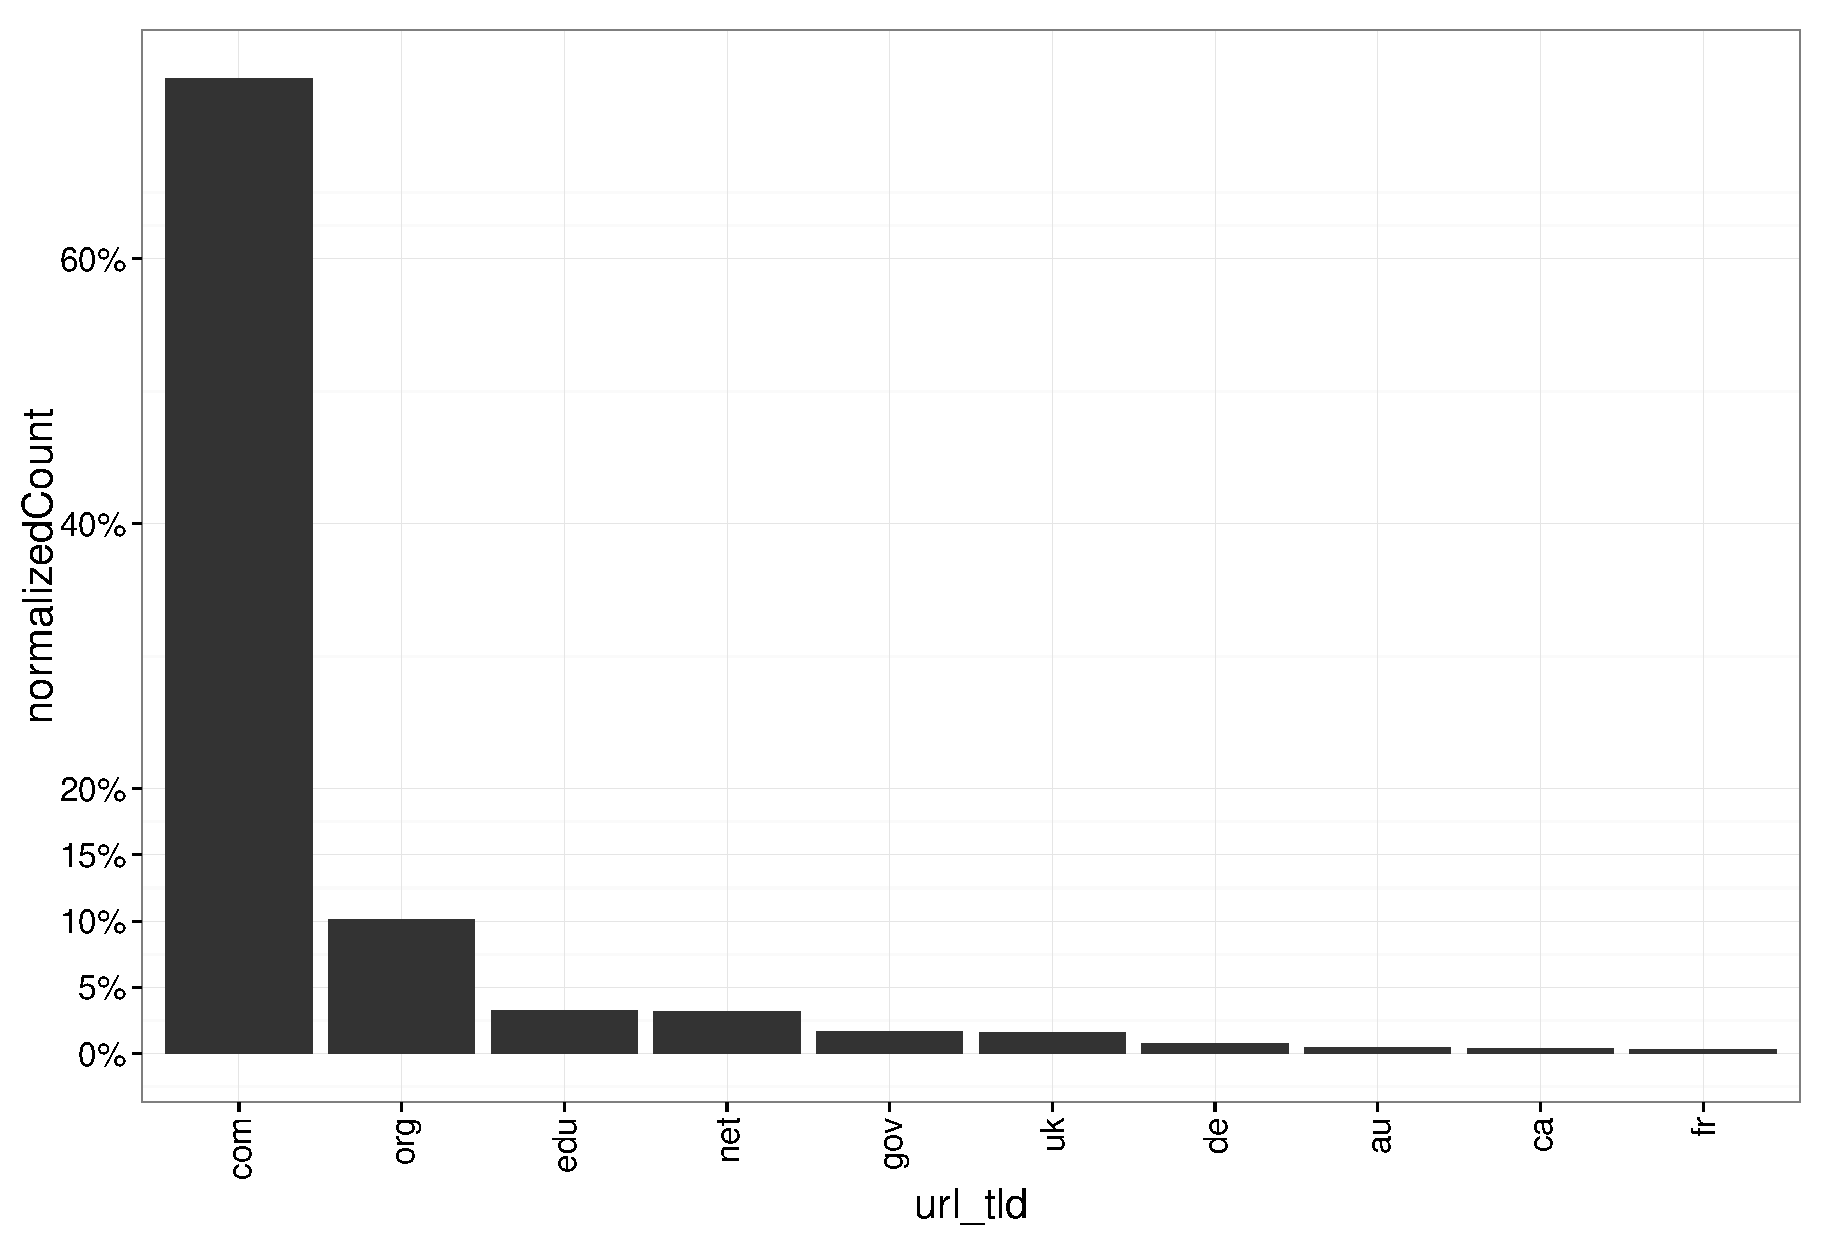
\includegraphics[width=1.1\textwidth]{plots/plot_tld_top10}}
\end{frame}

\begin{frame}{\insertsection: \insertsubsection}
    \makebox[\textwidth][c]{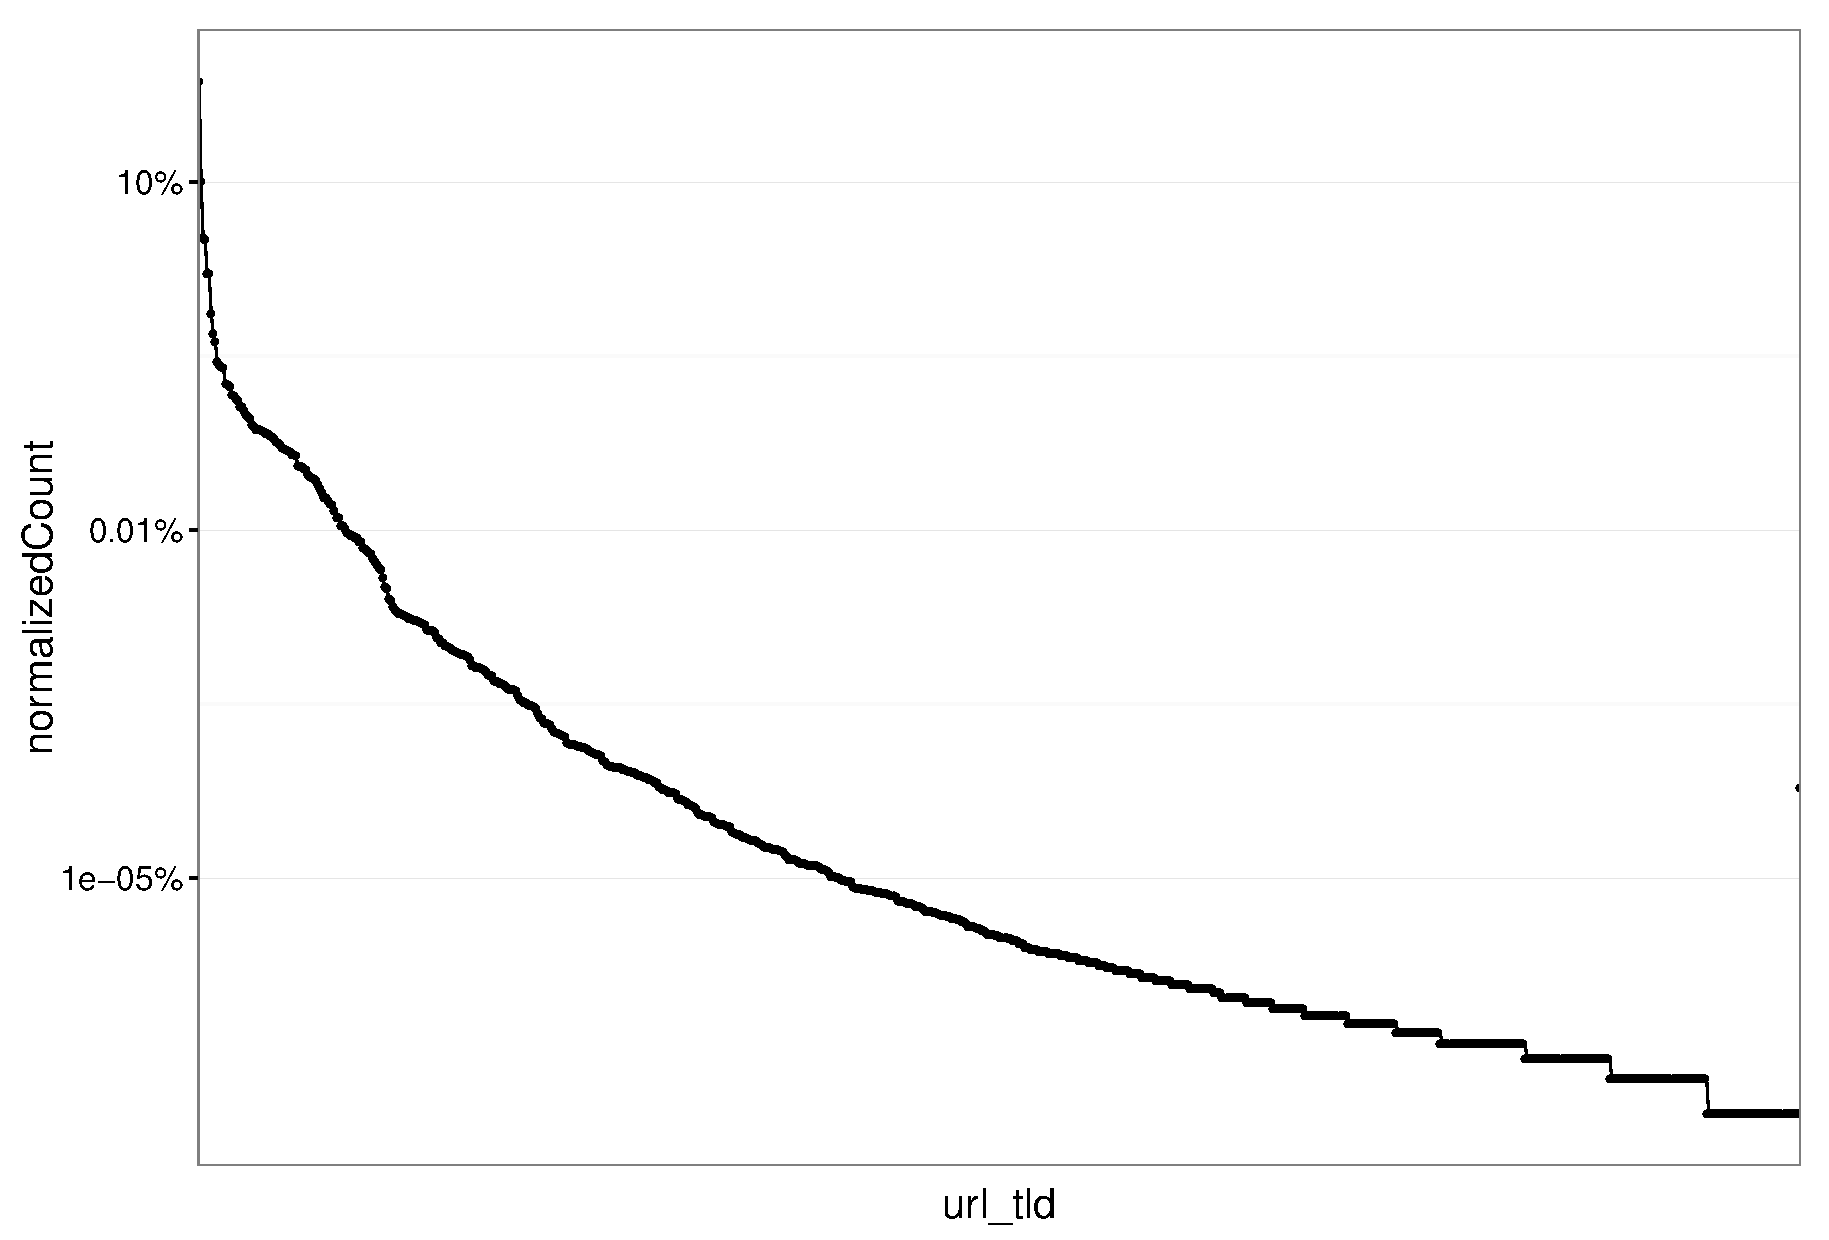
\includegraphics[width=1.1\textwidth]{plots/plot_tld}}
\end{frame}

\begin{frame}{\insertsection: \insertsubsection}
    \makebox[\textwidth][c]{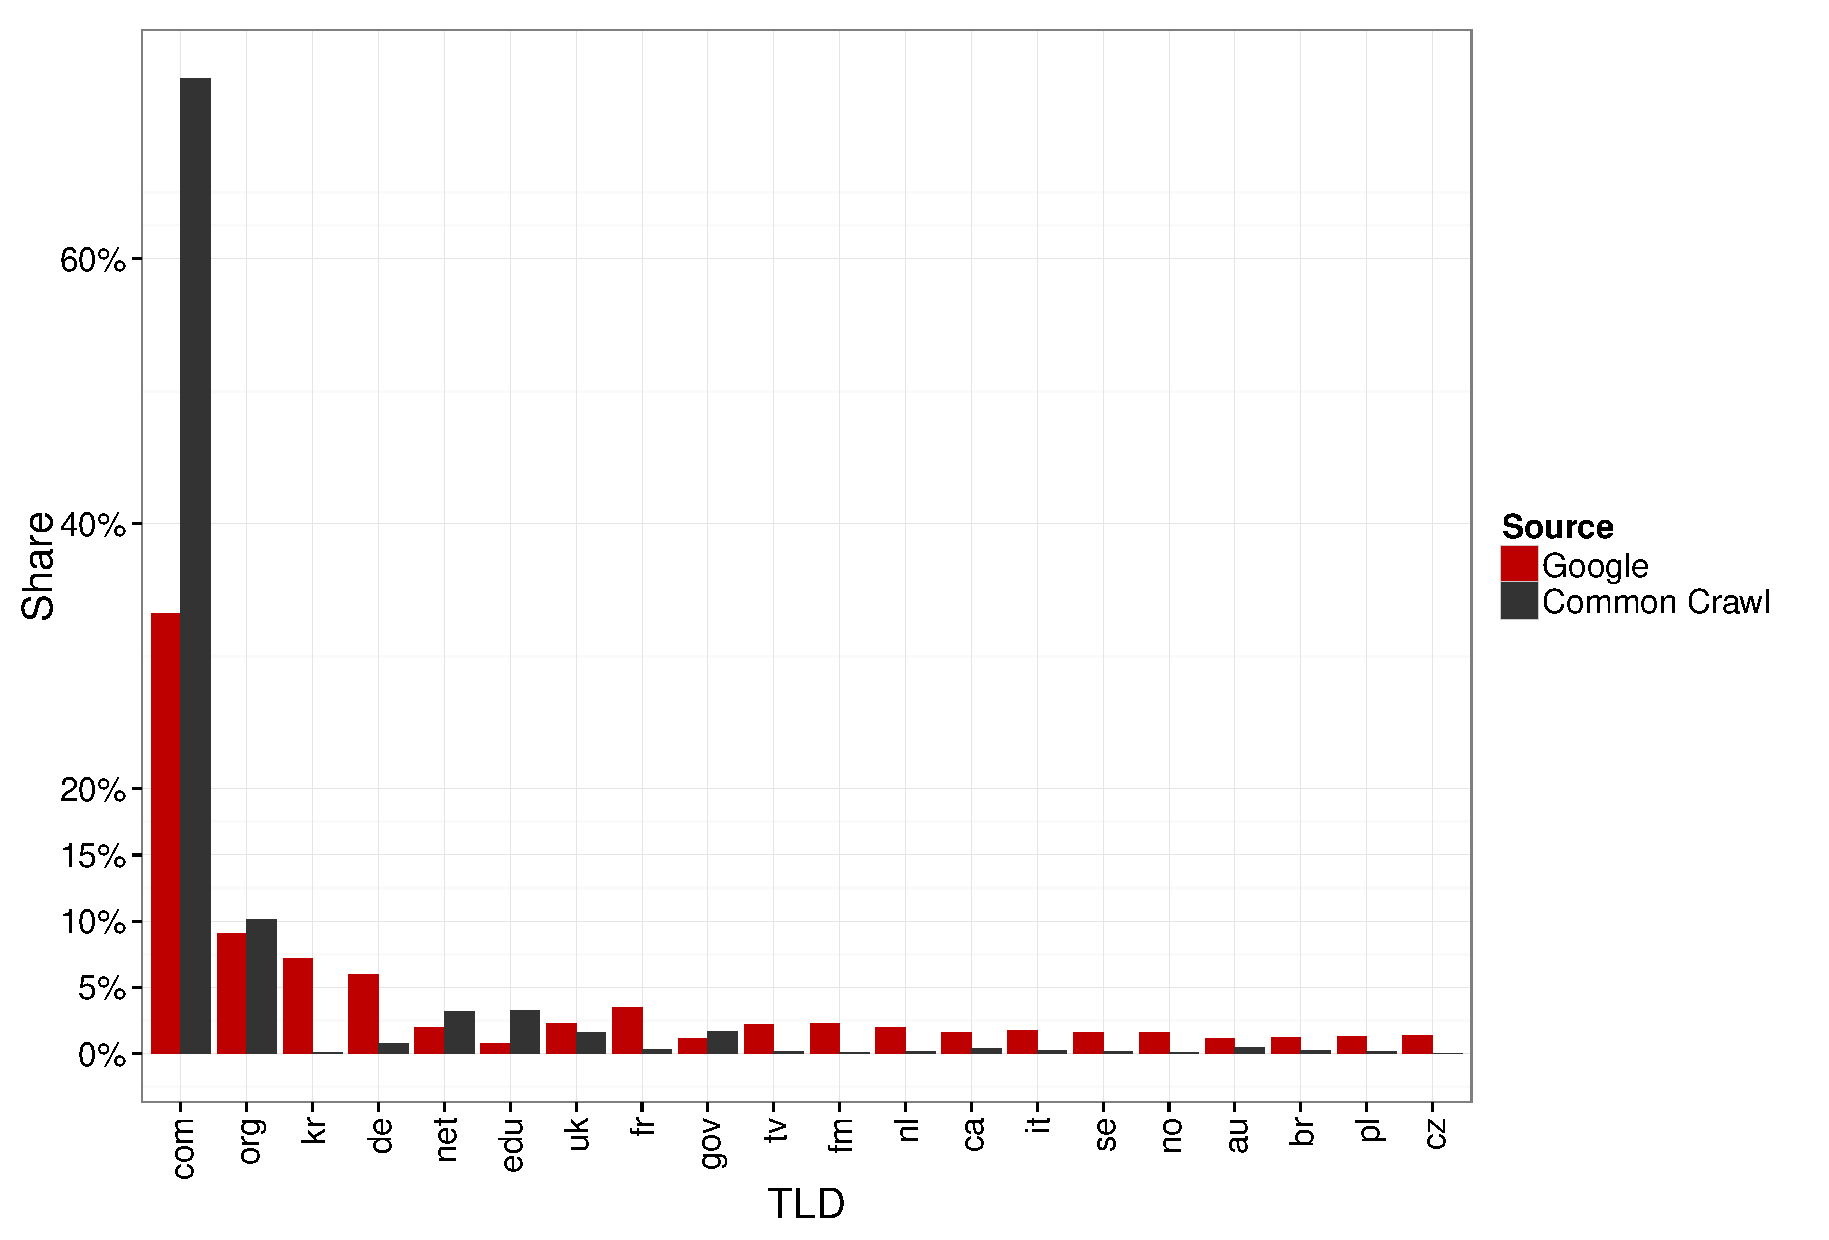
\includegraphics[width=1.1\textwidth]{plots/plot_tld_comparison}}
\end{frame}

\subsection{Public Suffix}
\begin{frame}{\insertsection: \insertsubsection}
    \makebox[\textwidth][c]{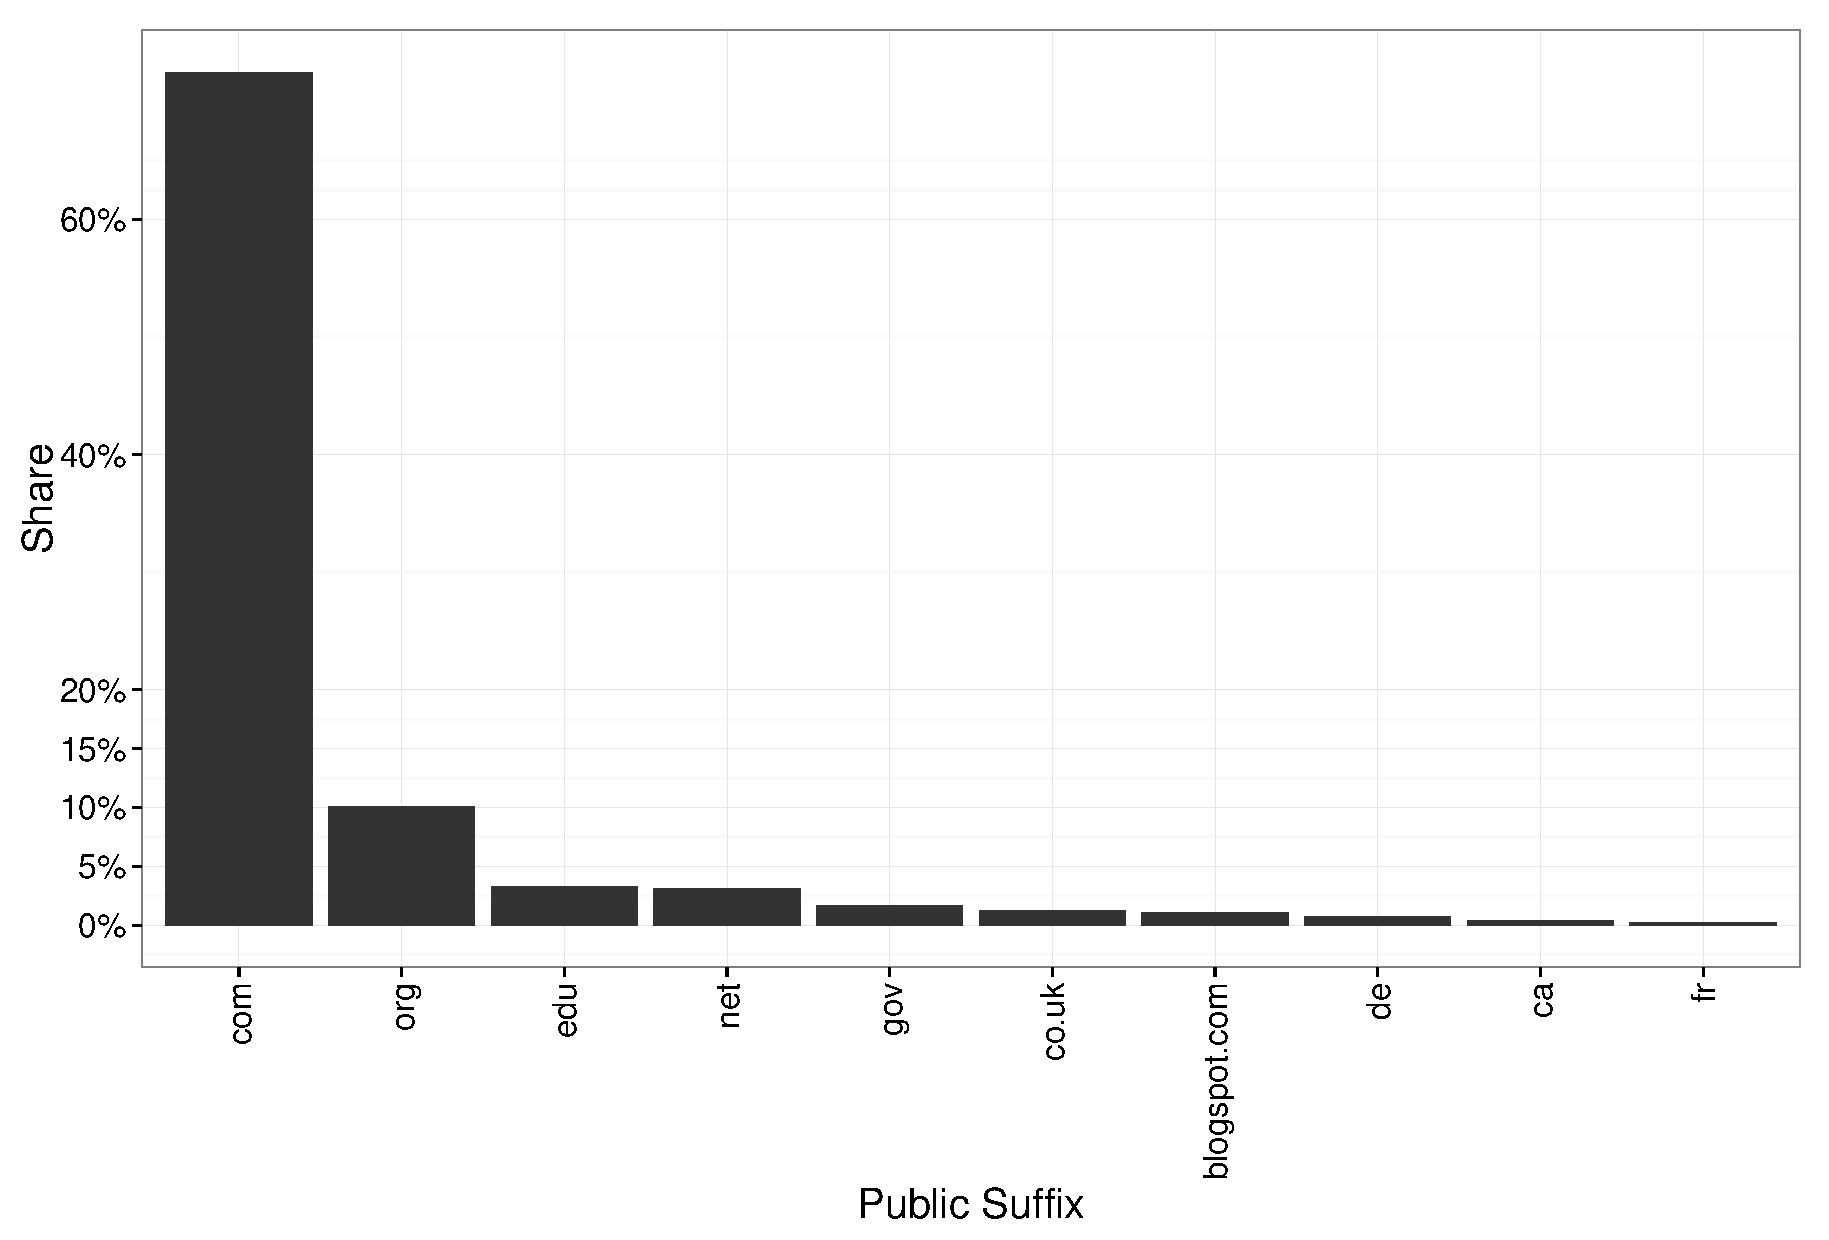
\includegraphics[width=1.1\textwidth]{plots/plot_pub_suffixes_top10}}
\end{frame}

\begin{frame}{\insertsection: \insertsubsection}
    \makebox[\textwidth][c]{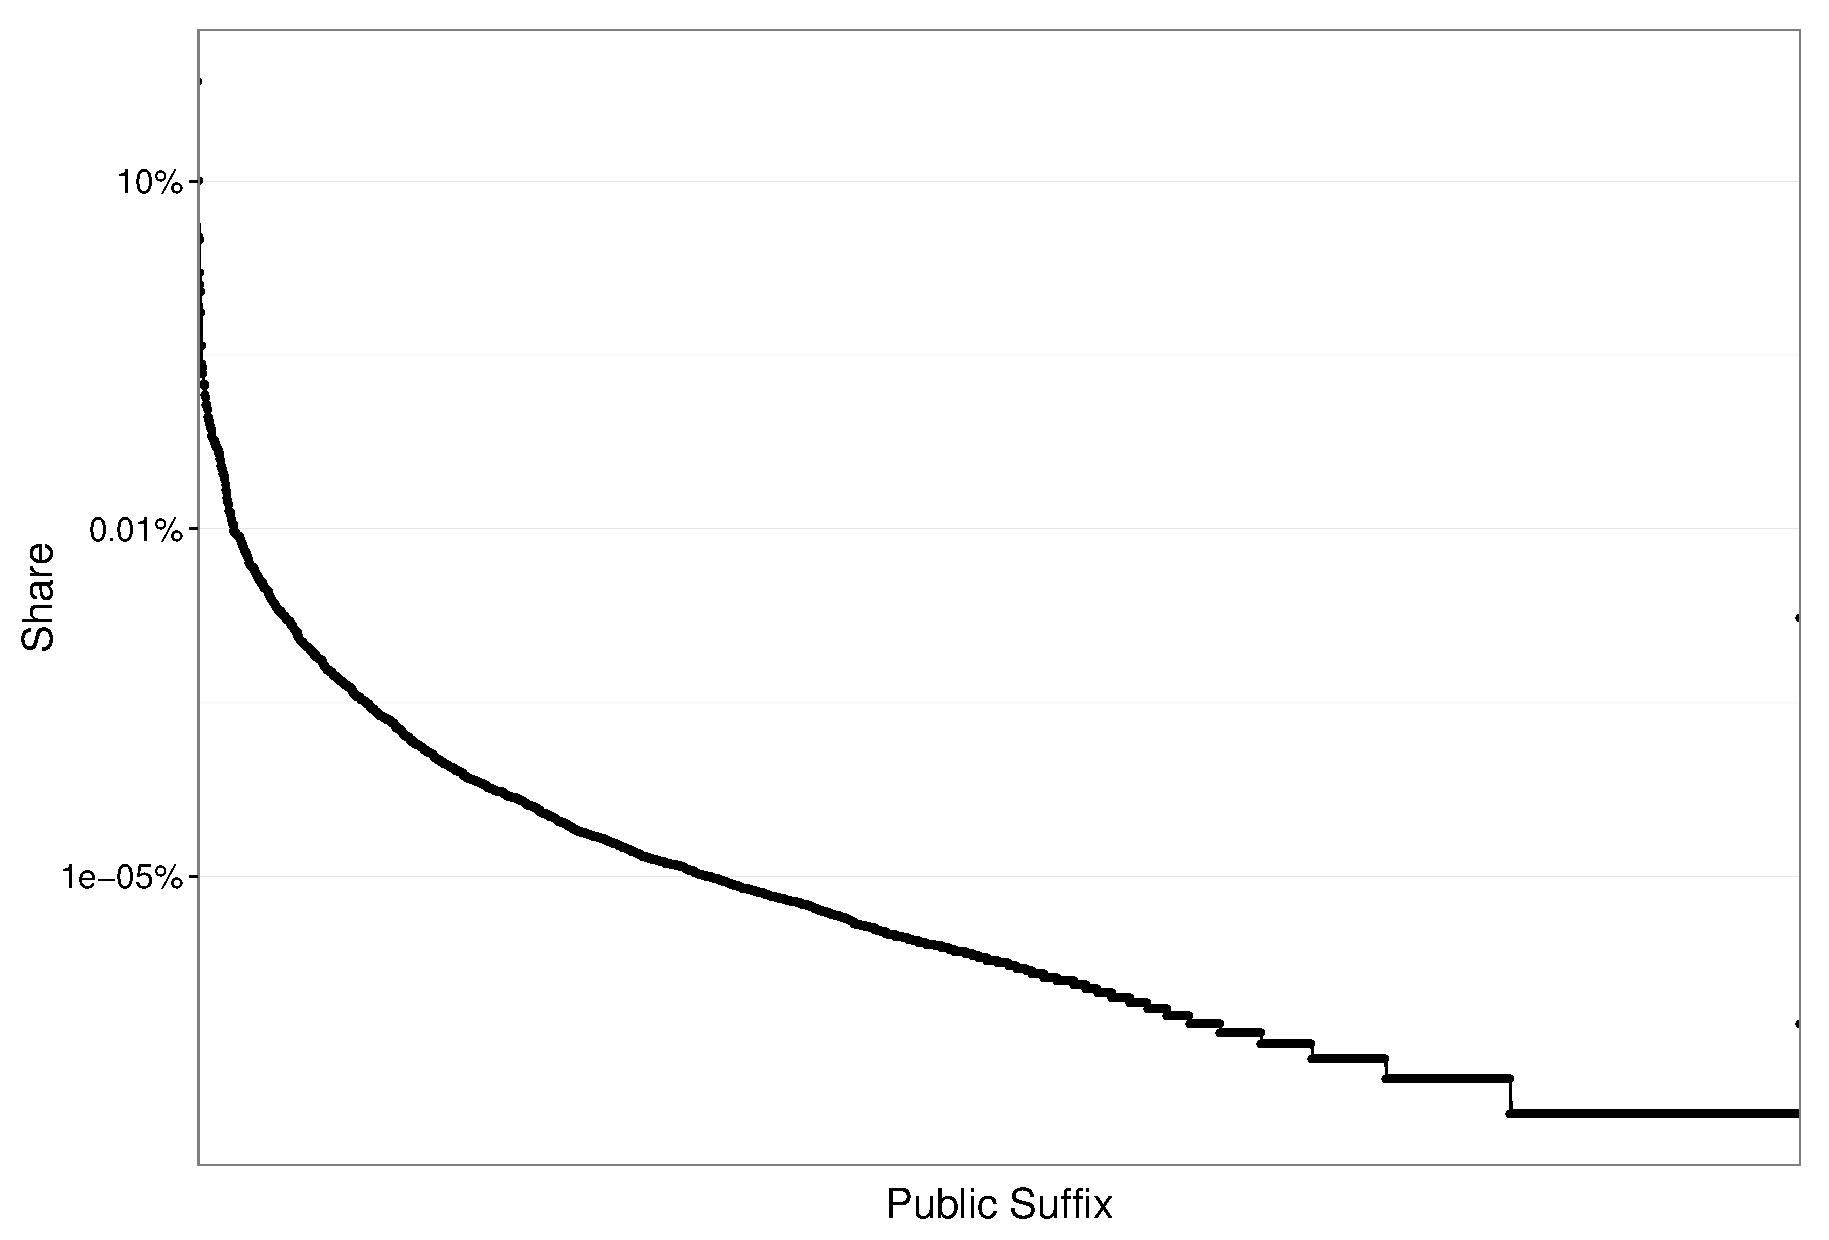
\includegraphics[width=1.1\textwidth]{plots/plot_pub_suffixes}}
\end{frame}

\subsection{Mime-Type}
\begin{frame}{\insertsection: \insertsubsection}
    \makebox[\textwidth][c]{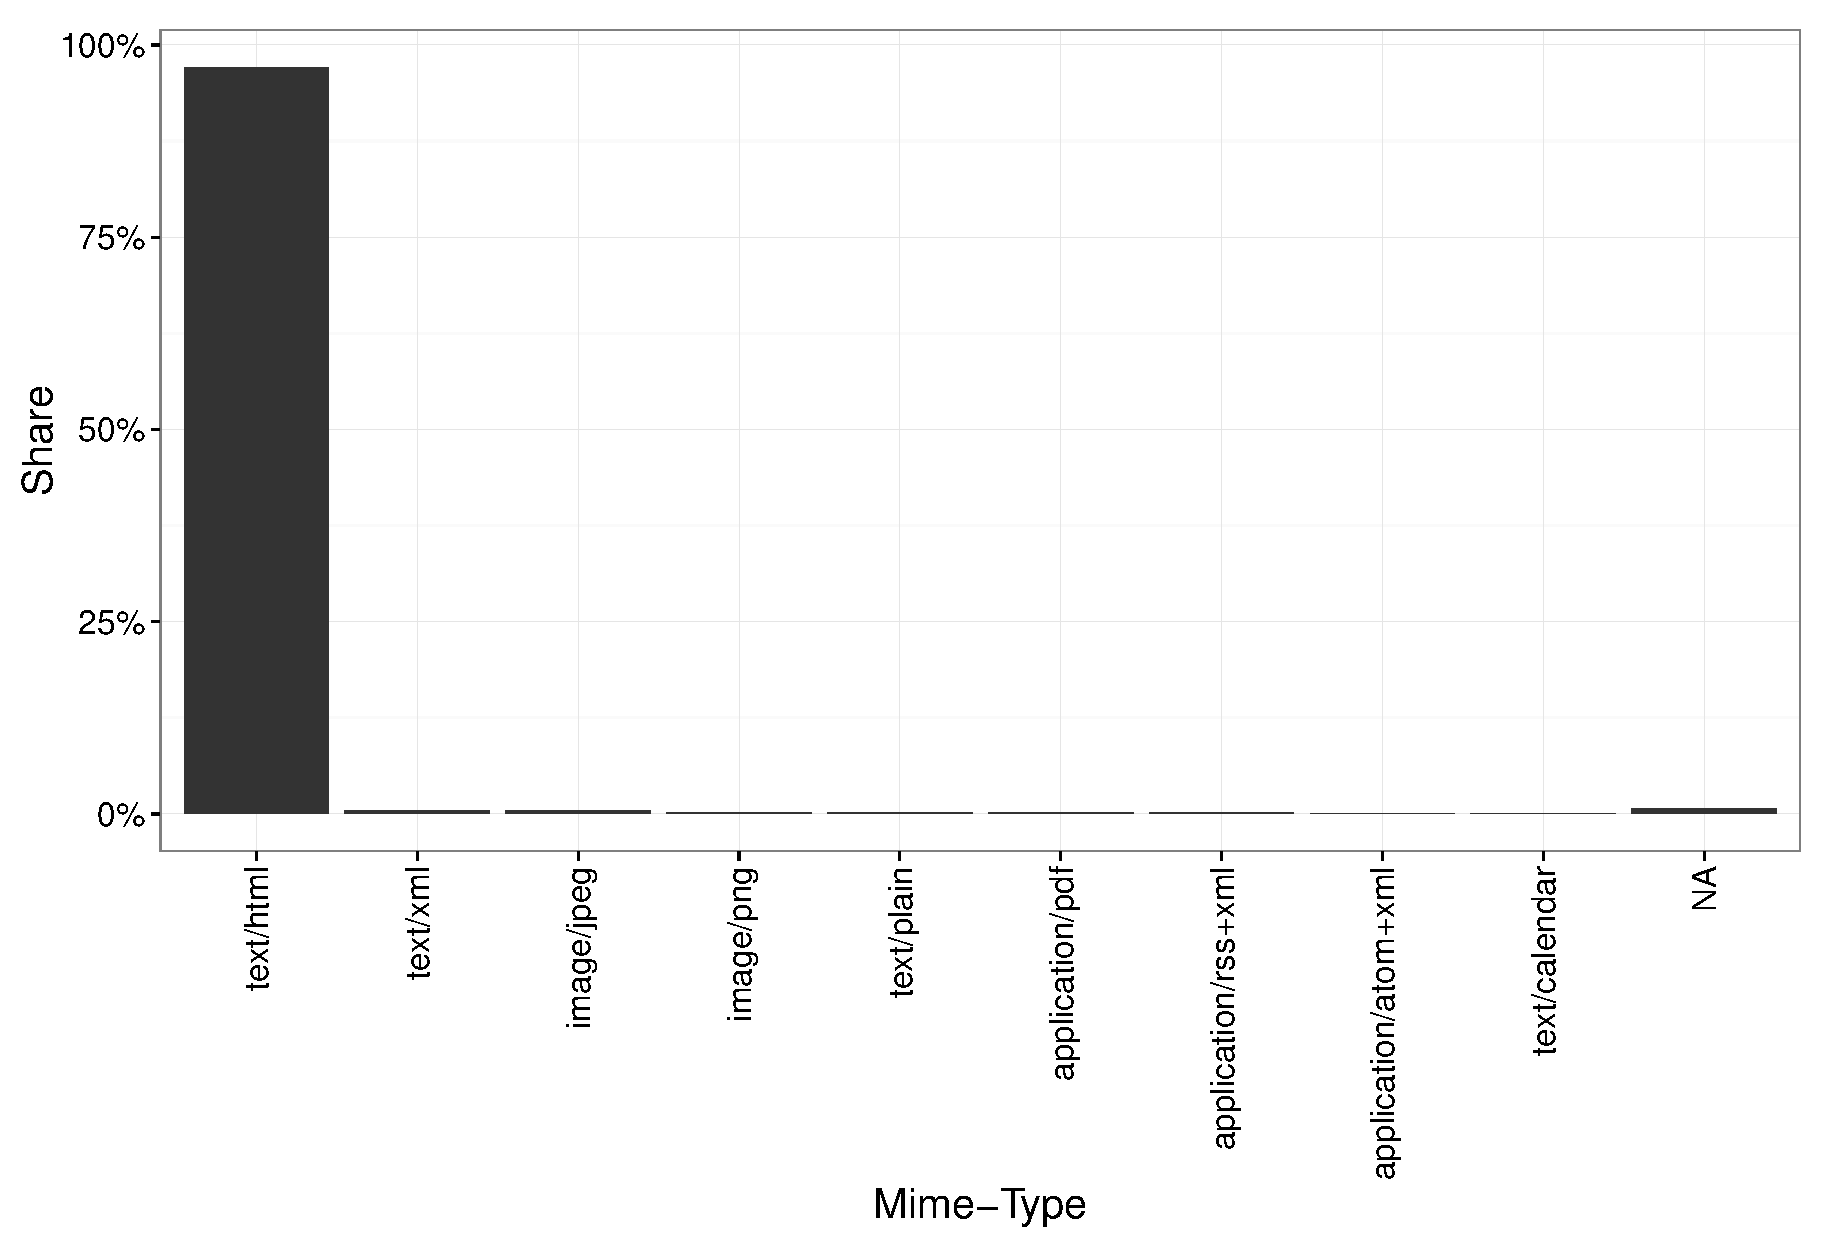
\includegraphics[width=1.1\textwidth]{plots/plot_mime}}
\end{frame}

\subsection{TLS}
\begin{frame}{\insertsection: \insertsubsection}
    \makebox[\textwidth][c]{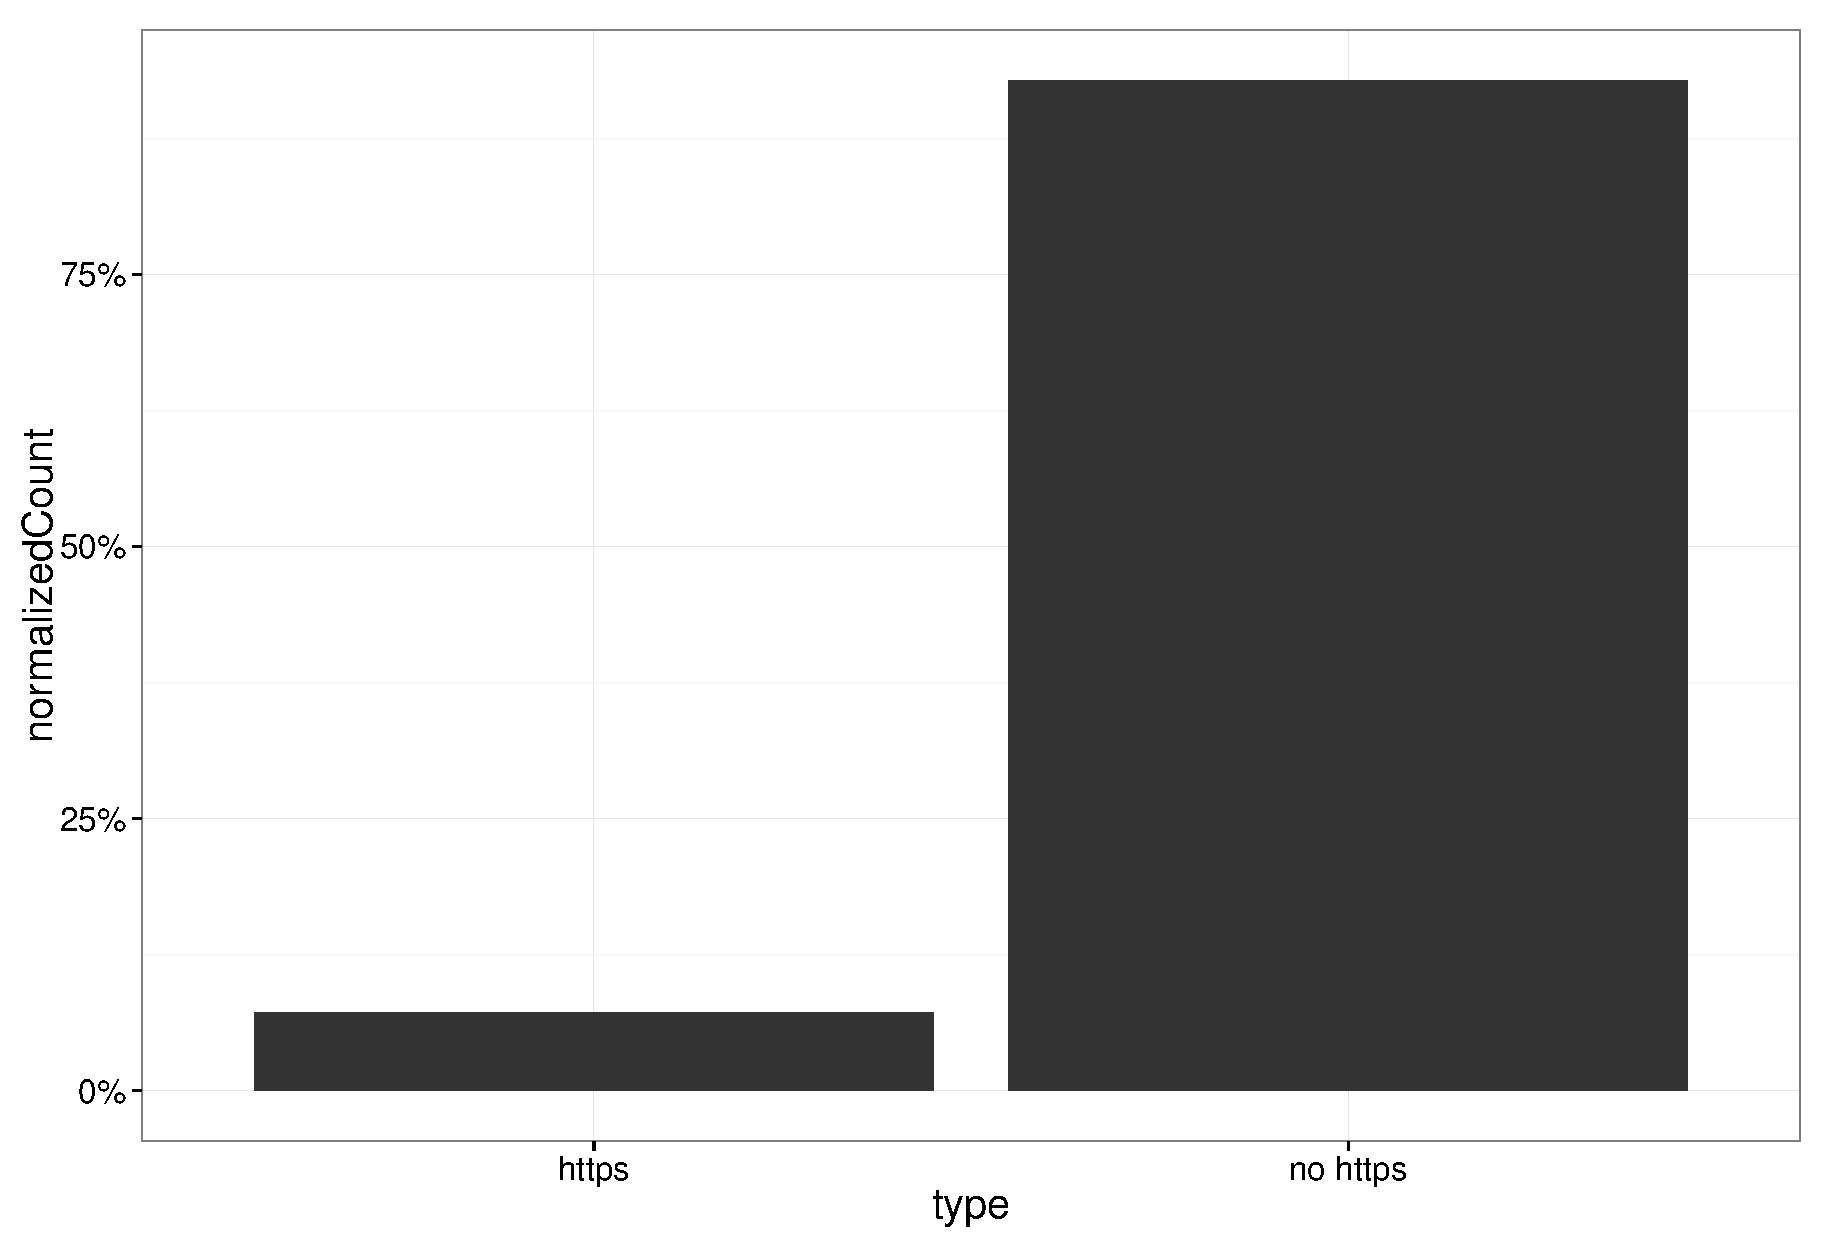
\includegraphics[width=1.1\textwidth]{plots/plot_https}}
\end{frame}

\subsection{Encoding}
\begin{frame}{\insertsection: \insertsubsection}
    \makebox[\textwidth][c]{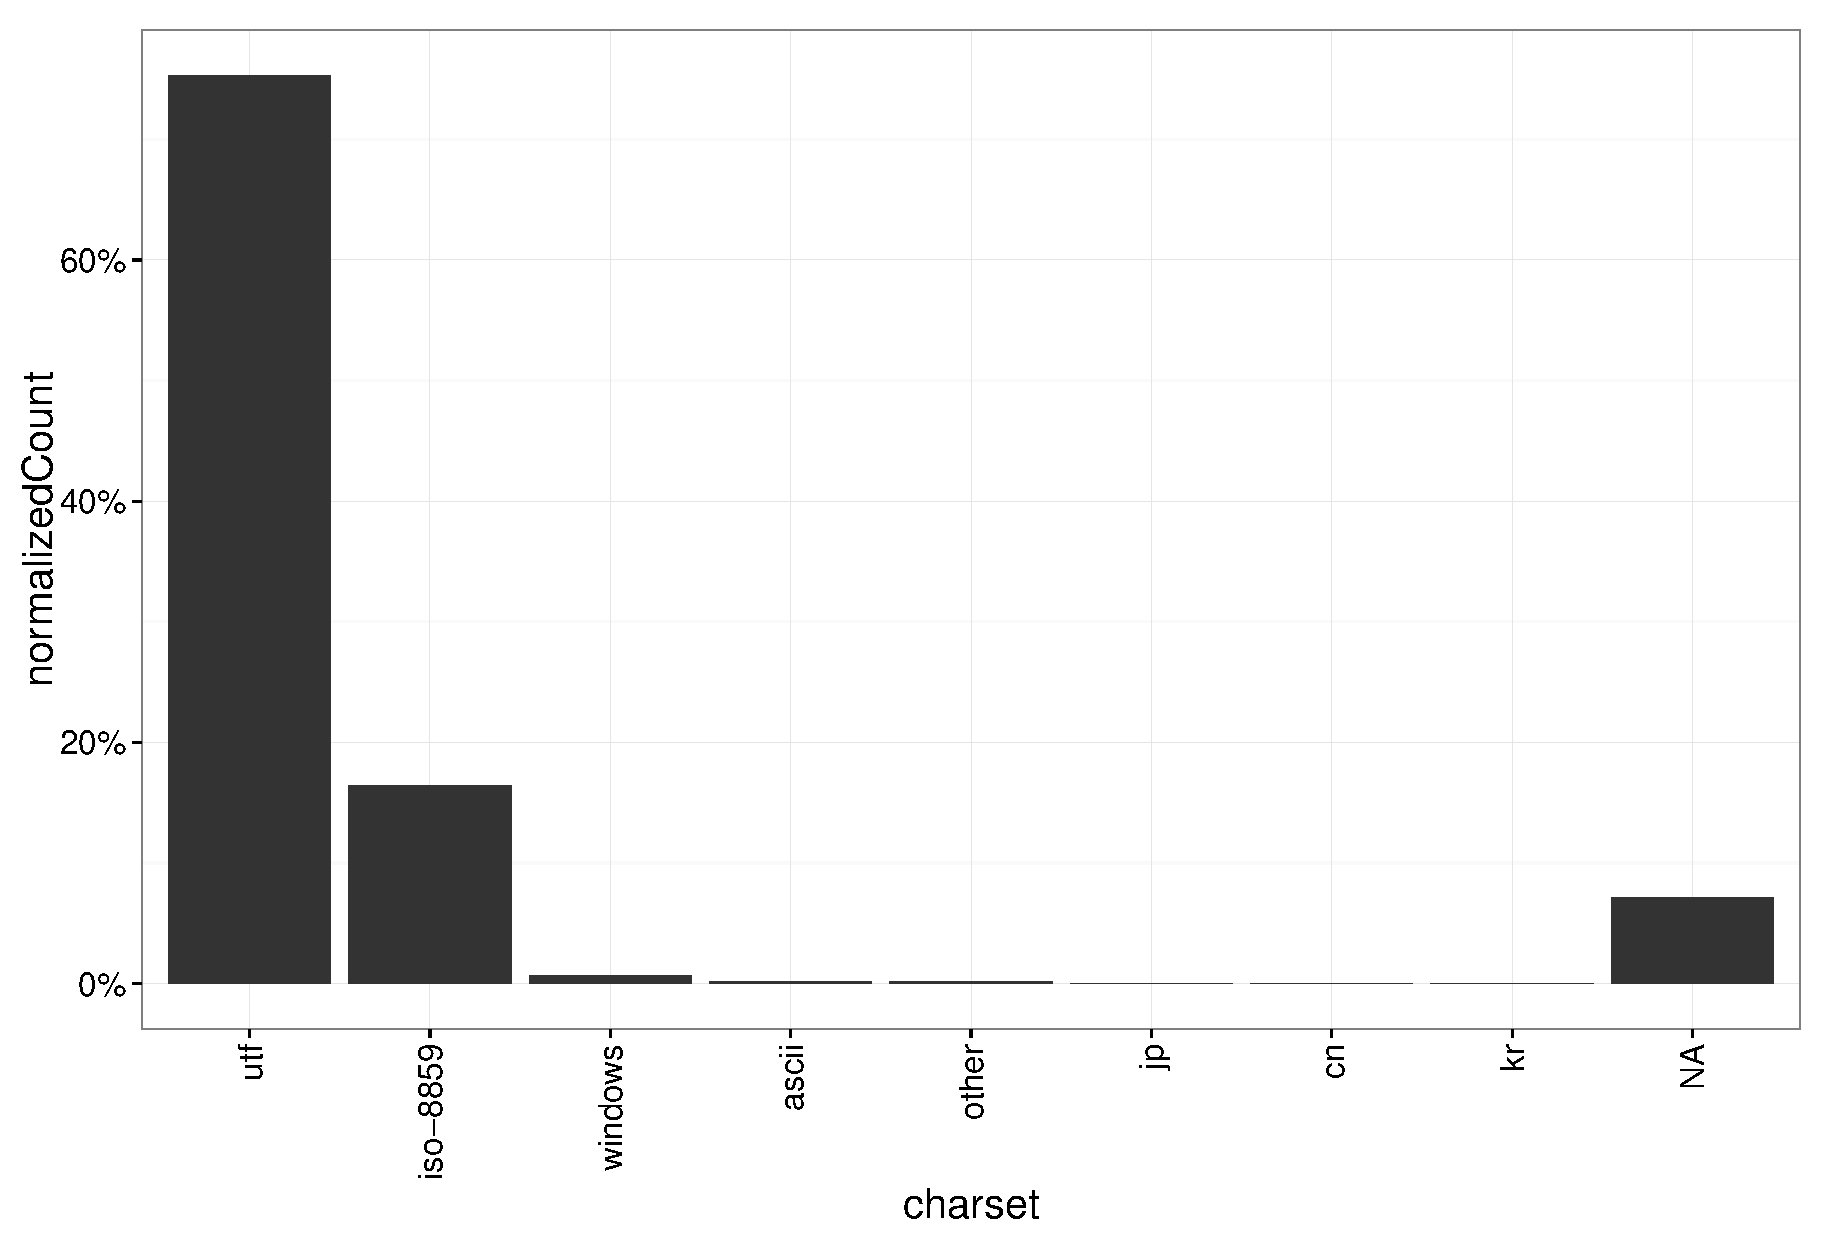
\includegraphics[width=1.1\textwidth]{plots/plot_charset}}
\end{frame}

\subsection{Server}
\begin{frame}{\insertsection: \insertsubsection}
    \makebox[\textwidth][c]{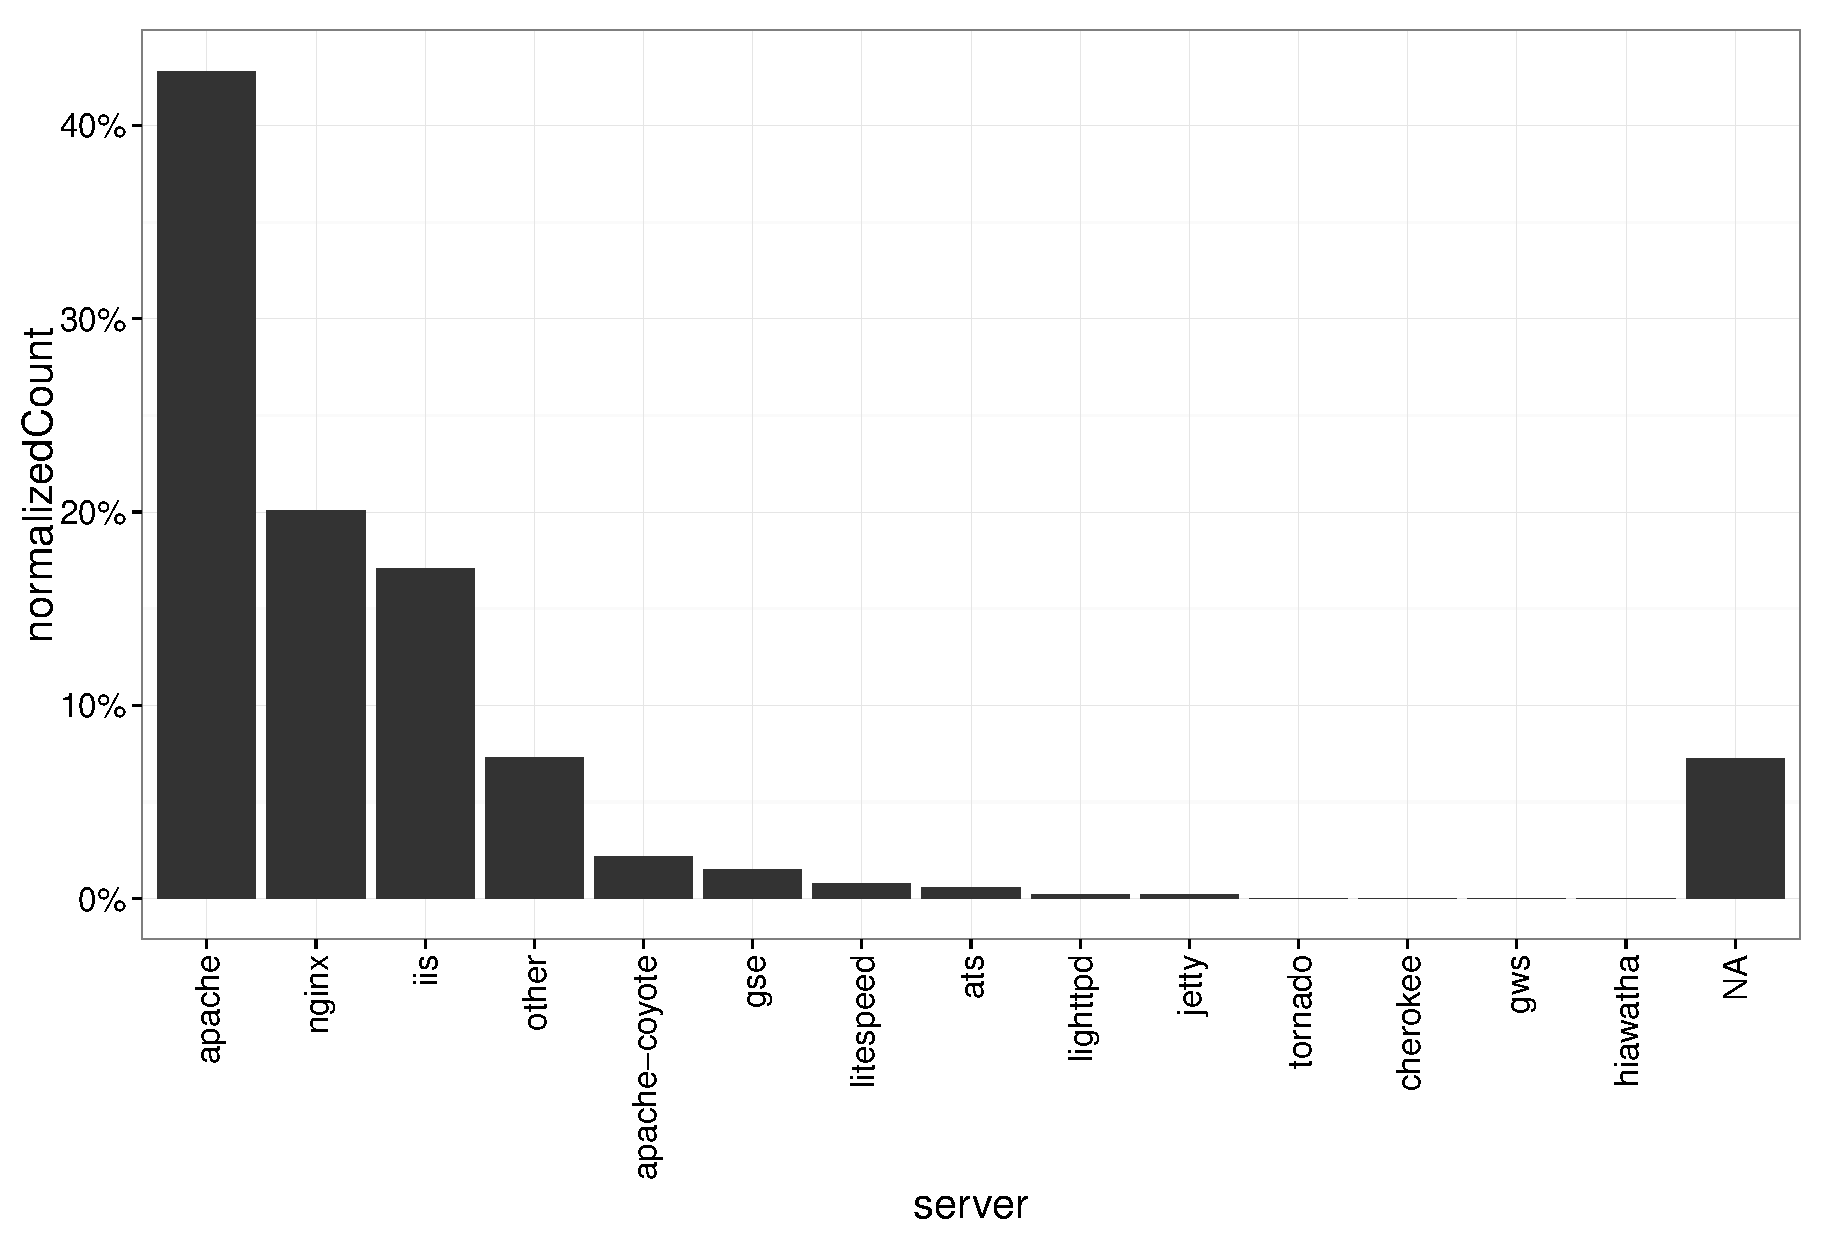
\includegraphics[width=1.1\textwidth]{plots/plot_server}}
\end{frame}


\section{Textextraktion}

\begin{frame}{\insertsection: Original}
    \centering{
        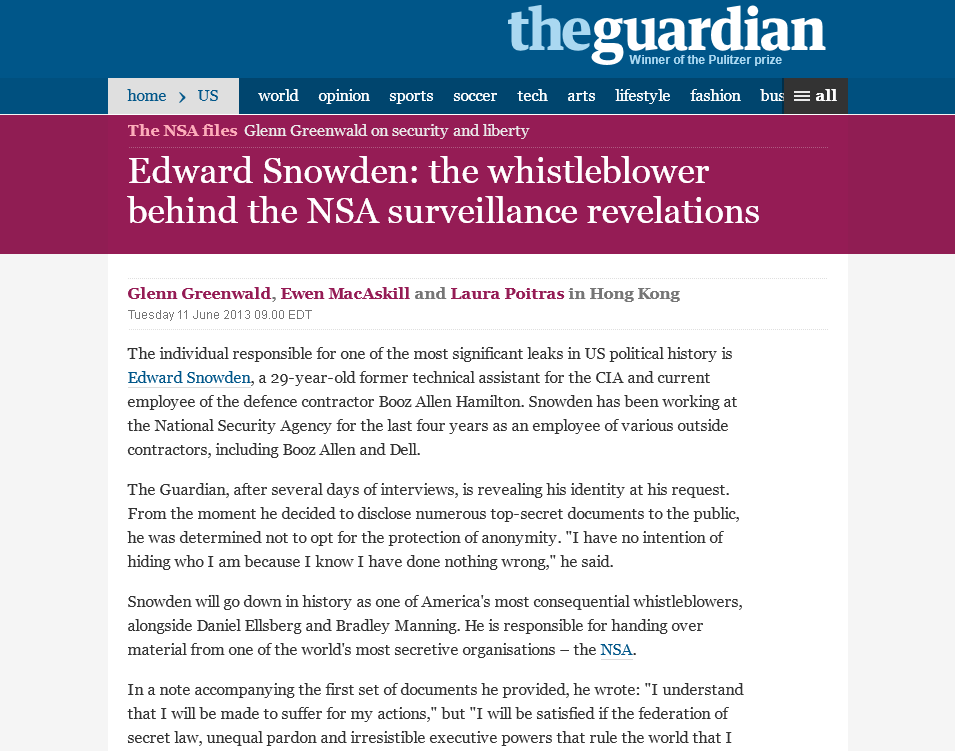
\includegraphics[trim=0 105px 0 0, clip=true, width=.9\textwidth]{images/guardian-website}
    }

    \scriptsize
    \vspace{.1cm}
    \url{http://www.theguardian.com/world/2013/jun/09/edward-snowden-nsa-whistleblower-surveillance}
\end{frame}

\begin{frame}{\insertsection: Common Crawl}
    \scriptsize
    Edward Snowden: the whistleblower behind the NSA surveillance revelations $|$ US news $|$ The Guardian
\end{frame}

\begin{frame}{\insertsection: jWarcEx}
    \scriptsize
    Skip to main content

    browse all sections close

    Glenn Greenwald on security and liberty

    Edward Snowden: the whistleblower behind the NSA surveillance revelations

    The 29-year-old source behind the biggest intelligence leak in the NSA's history explains his motives, his uncertain future and why he never intended on hiding in the shadows

    Q\&A with NSA whistleblower Edward Snowden: ``I do not expect to see home again''

    Glenn Greenwald, Ewen MacAskill and Laura Poitras in Hong Kong

    Tuesday 11 June 2013 09.00 EDT Last modified on Saturday 4 October 2014 10.54 EDT

    Sorry, your browser is unable to play this video.

    The individual responsible for one of the most significant leaks in US political history is Edward Snowden, a 29-year-old former technical assistant for the CIA and current employee of the defence contractor Booz Allen Hamilton. Snowden has been working at the National Security Agency for the last four years as an employee of various outside contractors, including Booz Allen and Dell.

    The Guardian, after several days of interviews, is revealing his identity at his request. From the moment he decided to disclose numerous top-secret documents to the public, he was determined not to opt for the protection of anonymity. ``I have no intention of hiding who I am because I know I have done nothing wrong,'' he said.

    (...)
\end{frame}

\begin{frame}{\insertsection: Mozilla Readability.js}
    \scriptsize
    Edward Snowden: the whistleblower behind the NSA surveillance revelations

    Laura Poitras

    The individual responsible for one of the most significant leaks in US political history is Edward Snowden, a 29-year-old former technical assistant for the CIA and current employee of the defence contractor Booz Allen Hamilton. Snowden has been working at the National Security Agency for the last four years as an employee of various outside contractors, including Booz Allen and Dell.

    The Guardian, after several days of interviews, is revealing his identity at his request. From the moment he decided to disclose numerous top-secret documents to the public, he was determined not to opt for the protection of anonymity. "I have no intention of hiding who I am because I know I have done nothing wrong," he said.

    (...)
\end{frame}

\begin{frame}{\insertsection: Common Crawl}
    \scriptsize
    Lance Armstrong, Tour de France champ, retires | abc7.com

    GO

    Personalize your weather by entering a location.

    Sorry, but the location you entered was not found. Please try again.

    Sections

    Traffic

    Video

    Los AngelesOrange CountyInland EmpireVentura CountyCalifornia

    Home

    Accuweather

    Traffic

    Video

    Photos

    Mobile Apps

    Local News Los AngelesOrange CountyInland EmpireVentura CountyCalifornia

    Map My News

    Shows Live Well Network

    Follow Us

    BREAKING NEWS

    (...)

    \vspace{.2cm}
    \url{http://abc7.com/archive/7962461}
\end{frame}

\begin{frame}{\insertsection: jWarcEx}
    \scriptsize
    Personalize your weather by entering a location.

    Sorry, but the location you entered was not found. Please try again.

    \vspace{.2cm}
    Sections Traffic Video Los AngelesOrange CountyInland EmpireVentura CountyCalifornia

    Home Accuweather Traffic Video Photos Mobile Apps

    Los AngelesOrange CountyInland EmpireVentura CountyCalifornia

    \quad BREAKING NEWS ABC shows live and on-demand -- Download the WATCH ABC app!

    \vspace{.2cm}
    Lance Armstrong, Tour de France champ, retires

    Seven-time Tour de France champion Lance Armstrong is retiring. He ends his career amidst a federal doping investigation.

    February 16, 2011 12:00:00 AM PST

    Seven-time Tour de France champion Lance Armstrong said he's retiring from the professional cycling circuit, this time for good. The 39-year-old is calling it ``Retirement 2.0'' and is making it clear there is no reset button this time.

    \vspace{.2cm}
    He says he wants to spend more time with his children and dedicate himself even more to the fight against cancer with his "Livestrong" Foundation.

    (...)

    \vspace{.2cm}
    \url{http://abc7.com/archive/7962461}
\end{frame}


\end{document}
